\ifx\wholebook\relax \else
% ------------------------

\documentclass[b5paper]{article}
\usepackage[nomarginpar
  %, margin=.5in
]{geometry}

\addtolength{\oddsidemargin}{-0.05in}
\addtolength{\evensidemargin}{-0.05in}
\addtolength{\textwidth}{0.1in}

\usepackage[en]{../../../prelude}

\setcounter{page}{1}

\begin{document}

\title{Red-black tree}

\author{Xinyu LIU
\thanks{{\bfseries Xinyu LIU} \newline
  Email: liuxinyu95@gmail.com \newline}
  }

\maketitle
\fi

\markboth{Red-black tree}{Elementary Algorithms}

\ifx\wholebook\relax
\chapter{Red-black tree}
\numberwithin{Exercise}{chapter}
\fi

\section{Introduction}
\label{sec:rbtree-introduction} \index{red-black tree}

In chapter 2, there is an example about binary search tree. We use it as a dictionary to count the word occurrence in a text. One may want to feed a address book to a binary search tree, and use it to look up the contact as below example program:

\lstset{frame = single}
\begin{lstlisting}[language=Bourbaki]
void addrBook(Input in) {
    bst<string, string> dict
    while (string name, string addr) = read(in)) {
        dict[name] = addr
    }
    loop {
        string name = read(console)
        var addr = dict[name]
        if (addr == null) {
            print("not found")
        } else {
            print("address is", addr)
        }
    }
}
\end{lstlisting}

Unlike the word counter program, this one performs poorly, especially when search names like Zara, Zed, Zulu, etc. This is because the address entries are typically listed in lexicographic order, i.e. the names are input in ascending order. If insert numbers 1, 2, 3, ..., $n$ to a binary search tree, it ends up like in figure \ref{fig:unbalanced-tree}. It is an extremely unbalanced binary search tree. The $lookup()$ is bound to $O(h)$ time for a tree with height $h$. When the tree is well balanced, the performance is $O(\lg n)$, where $n$ is the number of elements in the tree. But in this extreme case, the performance downgrades to $O(n)$. It is not better than list scan.

\begin{figure}[htbp]
  \centering
  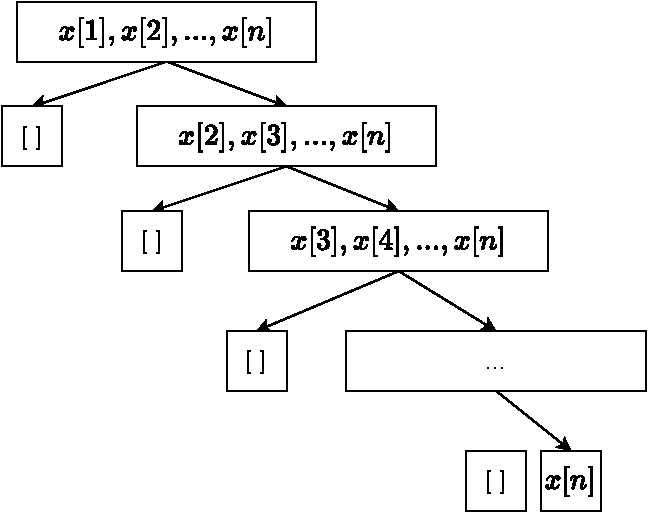
\includegraphics[scale=0.5]{img/unbalanced.ps}
  \caption{unbalanced tree}
  \label{fig:unbalanced-tree}
\end{figure}

\begin{Exercise}
\Question{For a big address entry list in lexicographic order, one may want to speed up the address book building with two concurrent tasks. One reads from the head, while the other reads from the tail. Till they meet at some middle point. What does the binary search tree look like? What if split the list into multiple sections to scale the concurrency?}
\Question{Find more cases to exploit a binary search tree, for example in figure \ref{fig:unbalanced-trees}.}
\end{Exercise}

\begin{figure}[htbp]
  \centering
  \subcaptionbox{}{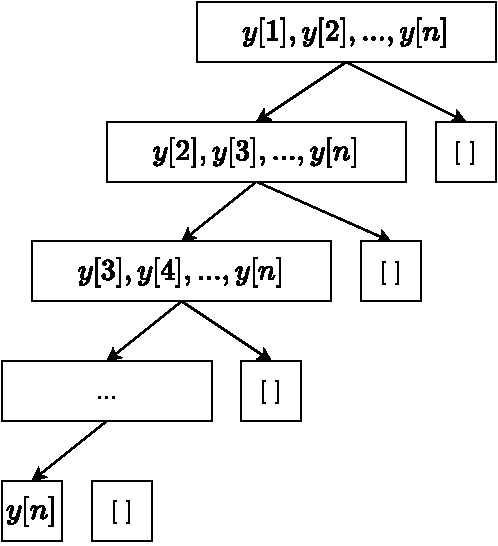
\includegraphics[scale=0.4]{img/unbalanced-2.ps}}
  \subcaptionbox{}{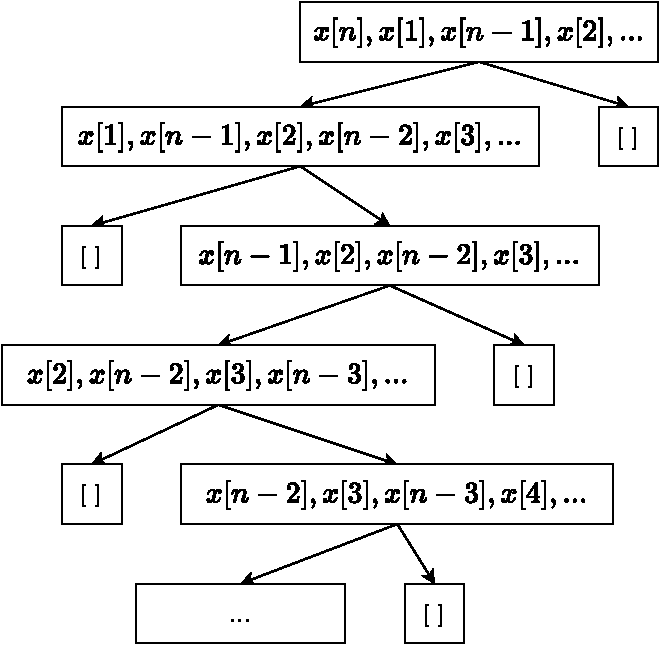
\includegraphics[scale=0.4]{img/unbalanced-zigzag.ps}} \\
  \subcaptionbox{}{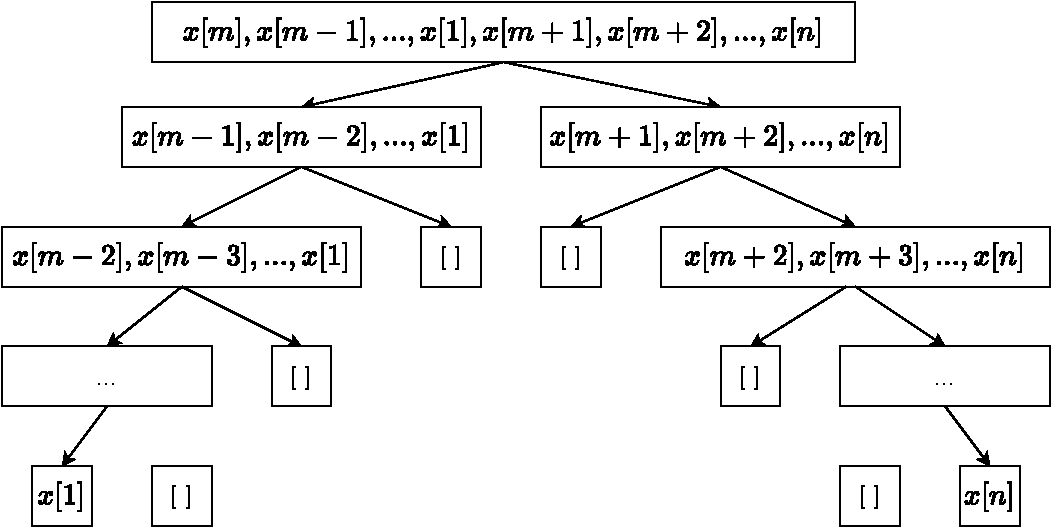
\includegraphics[scale=0.4]{img/unbalanced-3.ps}}
  \caption{Unbalanced trees}
  \label{fig:unbalanced-trees}
\end{figure}

\subsection{Balance}
To avoid extremely unbalanced case, we can shuffle the input(12.4 in \cite{CLRS}), however, there is situation that the input is fed from user, that we can not randomize the sequence. People developed solutions to make the tree balanced. They mostly rely on the rotation operation. Rotation changes the tree structure while maintain the elements ordering. This chapter introduces the red-black tree, the widely used self-adjusting balanced binary search tree. Next chapter is about AVL tree, another self-balanced tree. Chapter 8 introduce the splay tree, which adjust the tree in steps to make it balanced.

\subsection{Tree rotation}
\index{tree rotation}

\begin{figure}[htbp]
   \centering
   \setlength{\unitlength}{1cm}
   \begin{picture}(10, 4)
   \put(5, 2){$\Longleftrightarrow$}
   \subcaptionbox{}{\includegraphics[scale=0.4]{img/rotate-r.ps}}
   \subcaptionbox{}{\includegraphics[scale=0.4]{img/rotate-l.ps}}
   \end{picture}
   \\
   \begin{picture}(1, 0.5)\end{picture} %pad
   \caption{`left rotate' transforms the tree from left to right; `right rotate' is inverse.}
   \label{fig:tree-rotation}
\end{figure}

Tree rotation transforms the tree structure while keeping the in-order traverse result unchanged. There are multiple binary search trees generate the same ordered element sequence. Figure \ref{fig:tree-rotation} shows the tree rotation.

Tree rotation can be defined with pattern matching:

\be
\begin{array}{rcl}
rotate_l\ ((a, X, b), Y, c) & = & (a, X, (b, Y, c)) \\
rotate_l\ T & = & T \\
\end{array}
\ee

and

\be
\begin{array}{rcl}
rotate_r\ (a, X, (b, Y, c)) & = & ((a, X, b), Y, c)) \\
rotate_r\ T & = & T \\
\end{array}
\ee

We can also implement tree rotation imperatively. We need re-assign children and parent node references. When rotate, we pass both tree root $T$, and the node $x$ to apply rotation:

\begin{algorithmic}[1]
\Function{Left-Rotate}{$T, x$}
  \State $p \gets$ \Call{Parent}{$x$}
  \State $y \gets$ \Call{Right}{$x$} \Comment{assume $y \ne$ NIL}
  \State $a \gets$ \Call{Left}{$x$}
  \State $b \gets$ \Call{Left}{$y$}
  \State $c \gets$ \Call{Right}{$y$}
  \State \Call{Replace}{$x, y$}  \Comment{replace node $x$ with $y$}
  \State \Call{Set-Subtrees}{$x, a, b$} \Comment{Set $a, b$ as the sub-trees of $x$}
  \State \Call{Set-Subtrees}{$y, x, c$} \Comment{Set $x, c$ as the sub-trees of $y$}
  \If{$p = $ NIL}  \Comment{$x$ is the previous root}
    \State $T \gets y$
  \EndIf
  \State \Return $T$
\EndFunction
\end{algorithmic}

The \textproc{Right-Rotate} is symmetric, we leave it as exercise. The procedure \textproc{Replace}($x$, $y$) uses node $y$ to replace $x$:

\begin{algorithmic}[1]
\Function{Replace}{$x, y$}
  \State $p \gets$ \Call{Parent}{$x$}
  \If{$p$ = NIL} \Comment{$x$ is the root}
    \If{$y \ne$ NIL}
           \Call{Parent}{$y$} $\gets$ NIL
    \EndIf
  \ElsIf{\Call{Left}{$p$} $= x$}
    \State \Call{Set-Left}{$p$, $y$}
  \Else
    \State \Call{Set-Right}{$p$, $y$}
  \EndIf
  \State \Call{Parent}{$x$} $\gets$ NIL
\EndFunction
\end{algorithmic}

Procedure \textproc{Set-Subtrees}($x, L, R$) assigns $L$ as the left sub-tree of $x$, and $R$ as the right sub-tree.

\begin{algorithmic}[1]
\Function{Set-Children}{$x, L, R$}
  \State \Call{Set-Left}{$x, L$}
  \State \Call{Set-Right}{$x, R$}
\EndFunction
\end{algorithmic}

It further calls \textproc{Set-Left} and \textproc{Set-Right} to set the two sub-trees:

\begin{algorithmic}[1]
\Function{Set-Left}{$x, y$}
  \State \Call{Left}{$x$} $\gets y$
  \If{$y \ne$ NIL}
    \Call{Parent}{$y$} $\gets x$
  \EndIf
\EndFunction

\Statex

\Function{Set-Right}{$x, y$}
  \State \Call{Right}{$x$} $\gets y$
  \If{$y \ne$ NIL}
    \Call{Parent}{$y$} $\gets x$
  \EndIf
\EndFunction
\end{algorithmic}

We can see how pattern matching simplifies the tree rotation. Based on this idea, Okasaki developed the purely functional algorithm for red-black tree\cite{okasaki}.

\begin{Exercise}
\Question{Implement the \textproc{Right-Rotate} algorithm.}
\end{Exercise}

\section{Definition}
\index{red-black tree}

A red-black tree is a self-balancing binary search tree\cite{wiki-rbt}. It is essentially equivalent to 2-3-4 tree\footnote{Chapter 7 B-trees. For any 2-3-4 tree, there is at least one red-black tree has the same ordered data.}. By coloring the node red or black, and perform rotation, red-black tree provides a efficient way to keep the tree balanced. On top of the binary search tree definition, we label the node with a color. We say it is a red-black tree if the coloring satisfies the following 5 rules(\cite{CLRS} pp273):

\index{red-black tree!red-black properties}
\begin{enumerate}
\item Every node is either red or black.
\item The root is black.
\item Every leaf (NIL) is black.
\item If a node is red, then both sub-trees are black.
\item For each node, all paths from the node to descendant leaves contain the same number of black nodes.
\end{enumerate}

Why do they keep the red-black tree balanced? The key point is that, the longest path from root to leaf can not be as 2 times longer than the shortest path. Consider rule 4, there are not any two adjacent red nodes. Therefore, the shortest path contains only black nodes. Any longer path must have red one. In addition, rule 5 ensures all paths have the same number of black nodes. It eventually ensures any path is not 2 times longer than others\cite{wiki-rbt}. Figure \ref{fig:rbt-example-with-nil} gives an example red-black tree.

\begin{figure}[htbp]
  \centering
  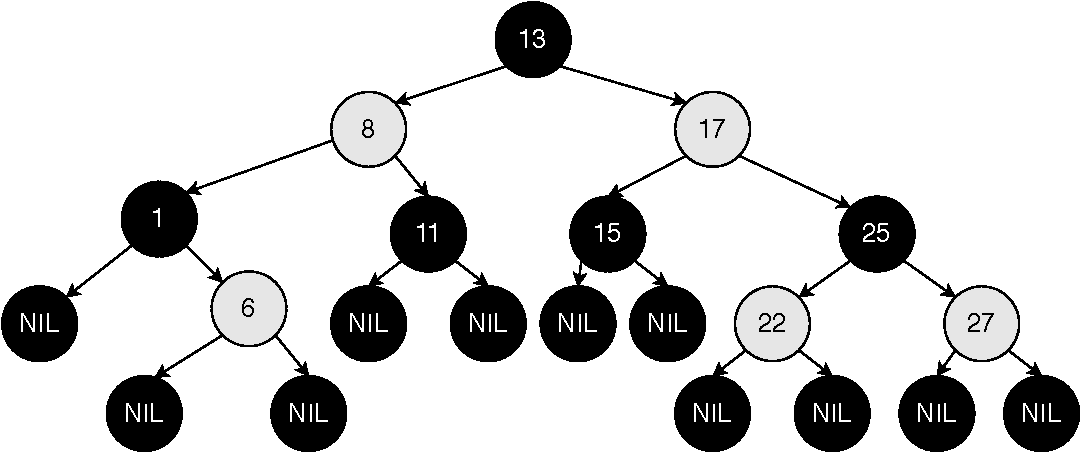
\includegraphics[scale=0.6]{img/rbt-example-with-nil.ps}
  \caption{A red-black tree}
  \label{fig:rbt-example-with-nil}
\end{figure}

As all NIL nodes are black, we can hide them in the figure, as shown in figure \ref{fig:rbt-example}. All operations including $lookup$, $min/max$, are same as the binary search tree. However, the $insert$ and $delete$ are special, as we need maintain the coloring rules.

\begin{figure}[htbp]
  \centering
  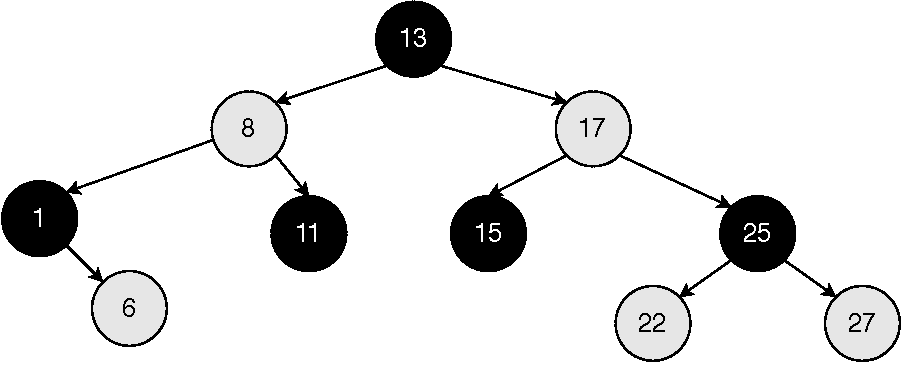
\includegraphics[scale=0.6]{img/rbt-example.ps}
  \caption{Hide the NIL nodes}
  \label{fig:rbt-example}
\end{figure}

Below example program adds the color field atop binary search tree definition:

\begin{Haskell}
data Color = R | B
data RBTree a = Empty
              | Node Color (RBTree a) a (RBTree a)
\end{Haskell}

\begin{Exercise}
\Question{Prove the height $h$ of a red-black tree of $n$ nodes is at most $2 \lg (n+1)$}
\end{Exercise}

\section{Insert}
\index{red-black tree!insert}

The idea of red-black tree $insert$ algorithm contains two steps. The first step is same as the binary search tree insertion. After that the tree may becomes unbalanced, we then fix it to resume the red-black tree coloring conditions in the second step. When insert a new element, we always make it a red node. Unless the new node is the root, we won't break any coloring rules except for the 4-th. This is because it may bring two adjacent red nodes. Okasaki finds there are 4 cases violate rule 4. All have two adjacent red nodes. They share a uniformed structure after fixing\cite{okasaki} as shown in figure \ref{fig:insert-fix}.

\begin{figure}[htbp]
  \centering
  \setlength{\unitlength}{1cm}
  \begin{picture}(15, 15)
    % arrows
    \put(4.5, 9.5){\vector(1, -1){1}}
    \put(4.5, 5){\vector(1, 1){1}}
    \put(10, 9.5){\vector(-1, -1){1}}
    \put(10, 5){\vector(-1, 1){1}}
    % graphics
    \put(0, 7){\includegraphics[scale=0.5]{img/insert-ll.ps}}
    \put(0, 0){\includegraphics[scale=0.5]{img/insert-lr.ps}}
    \put(7, 7){\includegraphics[scale=0.5]{img/insert-rr.ps}}
    \put(8.5, 0){\includegraphics[scale=0.5]{img/insert-rl.ps}}
    \put(2, 5){\includegraphics[scale=0.5]{img/insert-fixed.ps}}
  \end{picture}
  \caption{Fix 4 cases to the same structure in the center.}
  \label{fig:insert-fix}
\end{figure}

All 4 transformations move the redness one level up. When perform bottom-up recursive fixing, the last step will re-color the root as red. While rule 2 requires the root always be black. We need revert the root back to black finally. By using pattern matching, we can define a $balance$ function to fix the red-black tree. Denote the color as $\mathcal{C}$ with values black $\mathcal{B}$, and red $\mathcal{R}$. A none empty node is present as $T = (\mathcal{C}, T_l, k, T_r)$.

\be
\begin{array}{rcl}
balance\ (\mathcal{B}, (\mathcal{R}, (\mathcal{R}, A, x, B), y, C), z, D) & = & (\mathcal{R}, (\mathcal{B}, A, x, B), y, (\mathcal{B}, C, z, D)) \\
balance\ (\mathcal{B}, (\mathcal{R}, A, x, (\mathcal{R}, B, y, C), z, D))  & = & (\mathcal{R}, (\mathcal{B}, A, x, B), y, (\mathcal{B}, C, z, D)) \\
balance\ (\mathcal{B}, A, x, (\mathcal{R}, B, y, (\mathcal{R}, C, z, D))) & = & (\mathcal{R}, (\mathcal{B}, A, x, B), y, (\mathcal{B}, C, z, D))  \\
balance\ (\mathcal{B}, A, x, (\mathcal{R}, (\mathcal{R}, B, y, C), z, D)) & = & (\mathcal{R}, (\mathcal{B}, A, x, B), y, (\mathcal{B}, C, z, D))  \\
balance\ T & = & T \\
\end{array}
\ee

Where the last clause says if the tree is not in any 4 patterns, then we leave it unchanged. With $balance$ defined, we can modify the binary search tree $insert$ algorithm for red-black tree:

\be
insert(T, k) = makeBlack(ins(T, k))
\ee

where

\be
\begin{array}{rcl}
ins\ \nil\ k & = & (\mathcal{R}, \nil, k, \nil) \\
ins\ (\mathcal{C}, T_l, k', T_r)\ k & = & \begin{cases}
  k < k': & balance((ins(T_l, k), k', T_r)) \\
  k > k': & balance((T_l, k', ins(T_r, k))) \\
  \end{cases}
\end{array}
\ee

If the tree is empty, we create a red leaf of $k$; otherwise, let the sub-trees and the key be $T_l$, $T_r$, $k'$, we compare $k$ and $k'$, then recursively insert $k$ to a sub-tree. After that, we call $balance$ to fix the coloring, then force the root to be black finally.

\be
makeBlack\ (\mathcal{C}, T_l, k, T_r) = (\mathcal{B}, T_l, k, T_r)
\ee

Below it the corresponding example program:

\begin{Haskell}
insert t x = makeBlack $ ins t where
    ins Empty = Node R Empty x Empty
    ins (Node color l k r)
        | x < k     = balance color (ins l) k r
        | otherwise = balance color l k (ins r)
    makeBlack(Node _ l k r) = Node B l k r

balance B (Node R (Node R a x b) y c) z d =
                Node R (Node B a x b) y (Node B c z d)
balance B (Node R a x (Node R b y c)) z d =
                Node R (Node B a x b) y (Node B c z d)
balance B a x (Node R b y (Node R c z d)) =
                Node R (Node B a x b) y (Node B c z d)
balance B a x (Node R (Node R b y c) z d) =
                Node R (Node B a x b) y (Node B c z d)
balance color l k r = Node color l k r
\end{Haskell} %$

This program doesn't handle the case of duplicated keys. we can
either overwrite the key or drop the duplicated one.
Another option is to augment the data with a linked list(\cite{CLRS}, pp269).

Figure \ref{fig:insert-example} shows two red-black trees
built from feeding list 11, 2, 14, 1, 7, 15, 5, 8, 4 and 1, 2, ..., 8. The tree is well balanced even if we input an ordered list.

\begin{figure}[htbp]
  \centering
  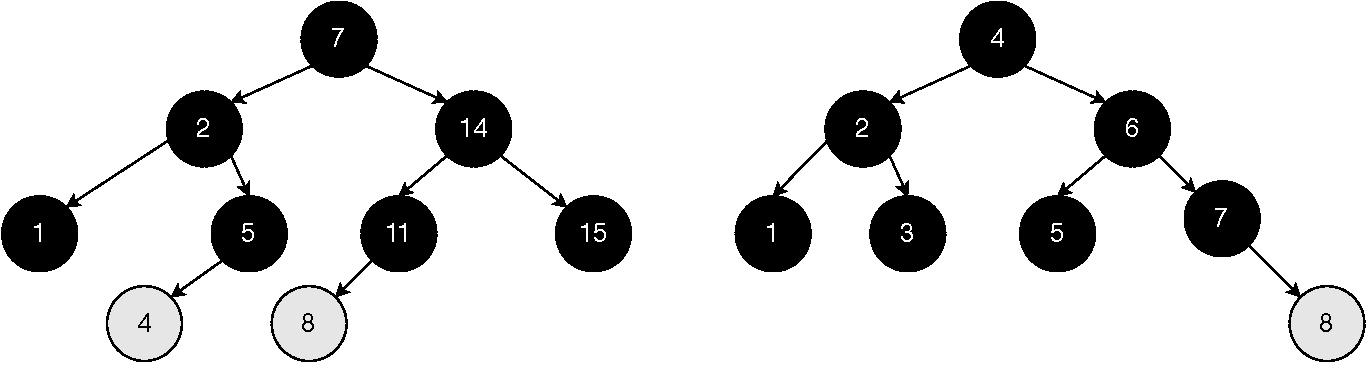
\includegraphics[scale=0.5]{img/insert-haskell.ps}
  \caption{insert results generated from two sequences of keys.} \label{fig:insert-example}
\end{figure}

This algorithm shows great simplicity by summarizing the uniform pattern
from the four different unbalanced cases. It is expressive over
the traditional tree rotation approach, that even in programming languages
which don't support pattern matching, the algorithm can still be
implemented by manually check the pattern. A Scheme/Lisp program
is available along with this book can be referenced as an example.

The insertion algorithm takes $O(\lg n)$ time to insert a key to
a red-black tree which has $n$ nodes.

\begin{Exercise}

\begin{itemize}
\item Write a program in an imperative language, such as
C, C++ or python to realize the same algorithm in this
section. Note that, because there is no language supported
pattern matching, you need to test the 4 different cases
manually.
\end{itemize}

\end{Exercise}

% ================================================================
%                 Deletion
% ================================================================

\section{Deletion}
\index{red-black tree!deletion}

Remind the deletion section in binary search tree. Deletion is
`imperative only' for red-black tree as well. In many cases,
the tree is often built just one time, and then
performs looking up frequently\cite{okasaki-blog}.

The purpose of this section is to show that red-black
tree deletion is possible in purely functional settings,
although it actually rebuilds the tree because trees are
read only in terms of purely functional data structure\footnote{Actually, the common part of the tree is reused. Most functional programming environments support this persistent feature.}.
In real world, it's up to the user (i.e. the
programmer) to adopt the proper solution. One option is to mark
the node be deleted with a flag, and later rebuild the tree
when the number of deleted nodes exceeds 50\%.

Deletion is more complex than insertion in both functional and
imperative settings, as there are more cases to fix.
Deletion may also violate the red black tree properties,
so we need fix it after the normal deletion as described
in binary search tree.

The problem only happens if you try to
delete a black node, because it will violate the last property
of red-black tree. The number of black
node in the path decreases so not all the paths contain the
same number of black node.

When delete a black node, we can resume the last red-black property
by introducing a 'doubly-black' concept(\cite{CLRS}, pp290). It means
that the although the node is deleted, the blackness is kept
by storing it in the parent node. If the parent node is red,
it turns to black, However, if it's already black, it
turns to `doubly-black'.

In order to express the 'doubly-black node', The definition
need some modification accordingly.

\lstset{language=Haskell}
\begin{lstlisting}
data Color = R | B | BB -- BB: doubly black for deletion
data RBTree a = Empty | BBEmpty -- doubly black empty
              | Node Color (RBTree a) a (RBTree a)
\end{lstlisting}

When deleting a node, we first perform the same binary search tree deleting
algorithm. After that, if the node to be sliced out is black, we
need fix the tree to keep the red-black properties. The
delete function is defined as the following.

\be
delete(T, k) = blackenRoot(del(T, k))
\ee

where

\be
del(T, k) = \left \{
  \begin{array}
  {r@{\quad:\quad}l}
  \phi & T = \phi \\
  fixBlack^2((\mathcal{C}, del(T_l, k), k', T_r)) & k < k' \\
  fixBlack^2((\mathcal{C}, T_l, k', del(T_r, k))) & k > k' \\
  \left \{
    \begin{array}{r@{\quad:\quad}l}
    mkBlk(T_r) & \mathcal{C} = \mathcal{B} \\
    T_r & otherwise
    \end{array}
  \right. & T_l = \phi \\
  \left \{
    \begin{array}{r@{\quad:\quad}l}
    mkBlk(T_l) & \mathcal{C} = \mathcal{B} \\
    T_l & otherwise
    \end{array}
  \right.  & T_r = \phi \\
  fixBlack^2((\mathcal{C}, T_l, k'', del(T_r, k''))) & otherwise
  \end{array}
\right.
\ee

The real deleting happens inside function $del$.
For the trivial case, that the tree is empty, the deletion
result is $\phi$; If the key to be deleted is less
than the key of the current node, we recursively
perform deletion on its left sub-tree; if it is bigger
than the key of the current node, then we recursively
delete the key from the right sub-tree; Because it
may bring doubly-blackness, so we need fix it.

If the key to be deleted is equal to the key of the
current node, we need splice it out. If one of its
children is empty, we just replace the node by
the other one and reserve the blackness of this
node. otherwise we cut and past the minimum
element $k''=min(T_r)$ from the right sub-tree.

Function $delete$ just forces the result tree of $del$
to have a black root. This is realized by function
$blackenRoot$.

\be
blackenRoot(T) = \left \{
  \begin{array}
  {r@{\quad:\quad}l}
  \phi & T = \phi \\
  (\mathcal{B}, T_l, k, T_r) & otherwise \\
  \end{array}
\right .
\ee

The $blackenRoot(T)$ function is almost same as the $makeBlack(T)$ function defined for insertion
except for the case of empty tree. This is only valid in
deletion, because insertion can't result an empty tree,
while deletion may.

Function $mkBlk$ is defined to reserved the blackness
of a node. If the node to be sliced isn't black, this function
won't be applied, otherwise, it turns a red node to black
and turns a black node to doubly-black. This function
also marks an empty tree $\phi$ to doubly-black empty $\Phi$.

\be
mkBlk(T) = \left \{
  \begin{array}
  {r@{\quad:\quad}l}
  \Phi & T = \phi \\
  (\mathcal{B}, T_l, k, T_r) & \mathcal{C} = \mathcal{R} \\
  (\mathcal{B}^2, T_l, k, T_r) & \mathcal{C} = \mathcal{B} \\
  T & otherwise
  \end{array}
\right .
\ee

where $\mathcal{B}^2$ denotes the doubly-black color.

Summarizing the above functions yields the following Haskell
program.

\begin{lstlisting}
delete t x = blackenRoot(del t x) where
    del Empty _ = Empty
    del (Node color l k r) x
        | x < k = fixDB color (del l x) k r
        | x > k = fixDB color l k (del r x)
        -- x == k, delete this node
        | isEmpty l = if color==B then makeBlack r else r
        | isEmpty r = if color==B then makeBlack l else l
        | otherwise = fixDB color l k' (del r k') where k'= min r
    blackenRoot (Node _ l k r) = Node B l k r
    blackenRoot _ = Empty

makeBlack (Node B l k r) = Node BB l k r -- doubly black
makeBlack (Node _ l k r) = Node B l k r
makeBlack Empty = BBEmpty
makeBlack t = t
\end{lstlisting}

The final attack to the red-black tree deletion algorithm is to
realize the $fixBlack^2$ function. The purpose of this function
is to eliminate the `doubly-black' colored node by rotation and
color changing. There are three cases. In every case, the doubly black
node can either be normal node, or doubly black empty node $\Phi$.
Let's examine these three cases one by one.

\subsection{The sibling of the doubly black node is black, and it has one red child}

In this situation, we can fix the doubly-blackness with one rotation.
Actually there are 4 different sub-cases, all of them can be transformed
to one uniformed pattern. They are shown in the figure \ref{fig:del-case1}.

\begin{figure}[htbp]
   \centering
   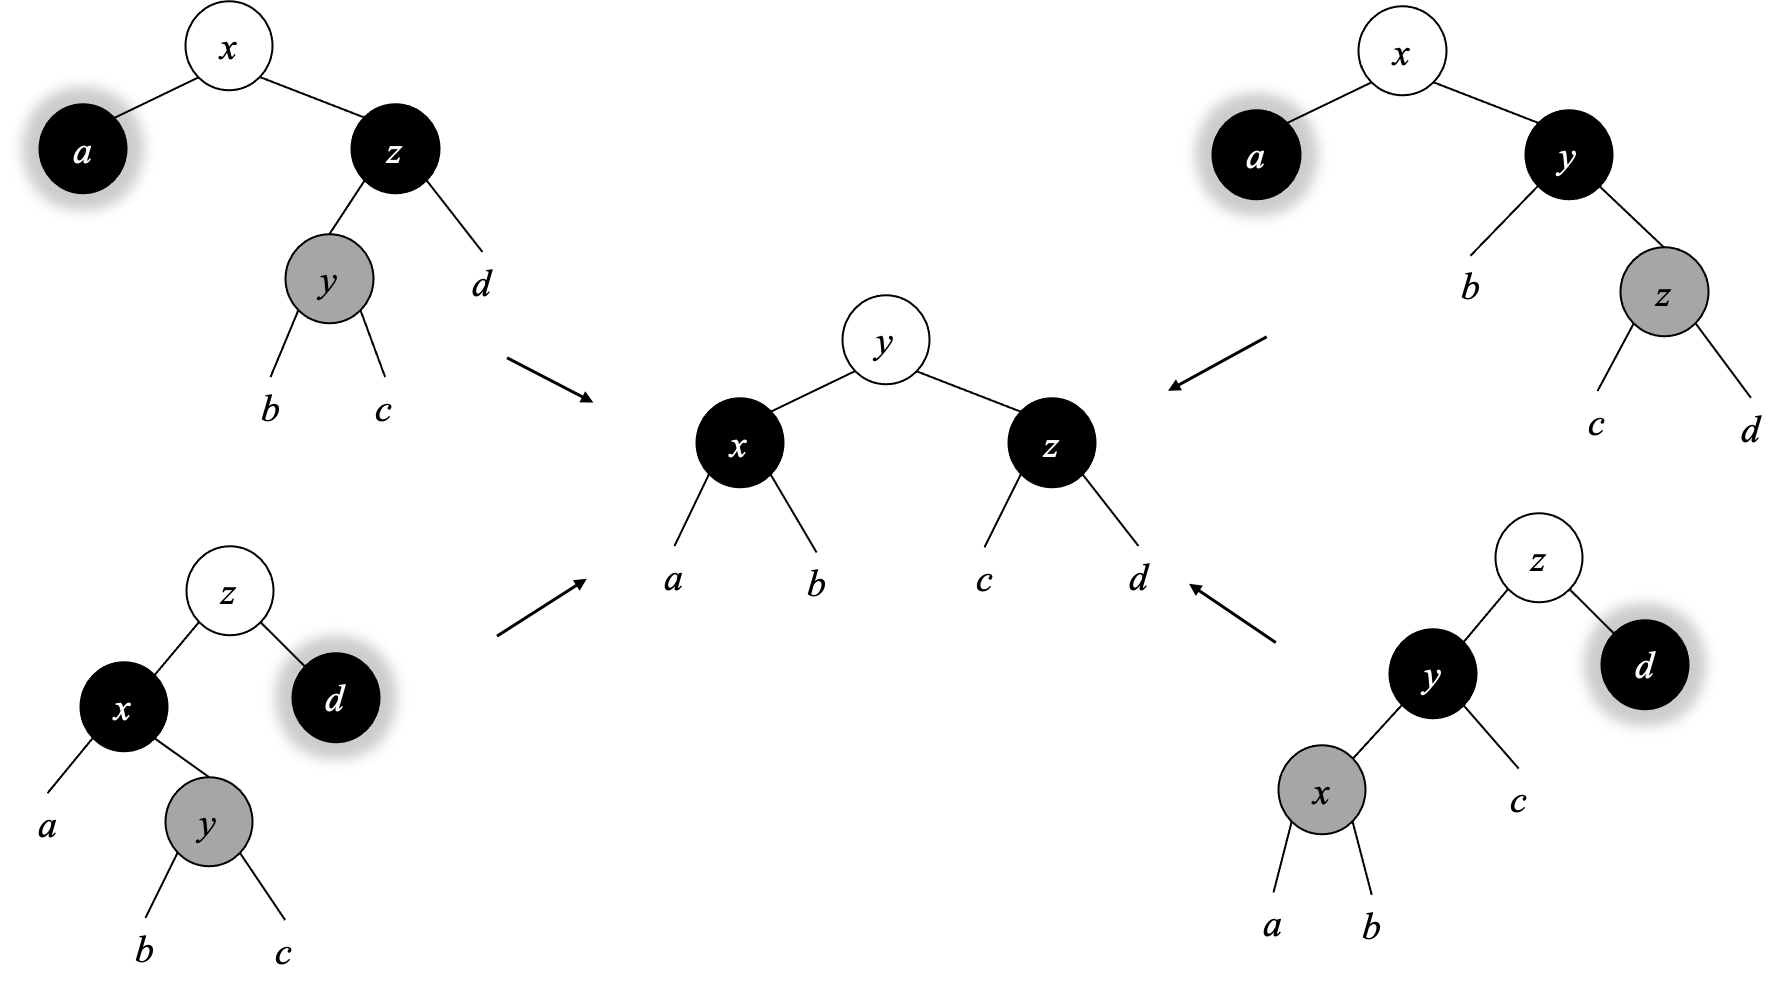
\includegraphics[scale=0.4]{img/del-case1.eps}
   \caption{Fix the doubly black by rotation, the sibling of the doubly-black node is black, and it has one red child.} \label{fig:del-case1}
\end{figure}

The handling of these 4 sub-cases can be realized with pattern matching.

\be
fixBlack^2(T) = \left \{
  \begin{array}
  {r@{\quad:\quad}l}
  (\mathcal{C}, (\mathcal{B}, mkBlk(A), x, B), y, (\mathcal{B}, C, z, D)) & p 1.1 \\
  (\mathcal{C}, (\mathcal{B}, A, x, B), y, (\mathcal{B}, C, z, mkBlk(D))) & p 1.2 \\
  \end{array}
\right .
\label{eq:db-case-1}
\ee

where $p 1.1$ and $p 1.2$ each represent 2 patterns as the following.

\[
p 1.1 : \left \{ \begin{array}{l}
  T = (\mathcal{C}, A, x, (\mathcal{B}, (\mathcal{R}, B, y, C), z, D)) \land color(A) = \mathcal{B}^2 \\
  \lor \\
  T = (\mathcal{C}, A, x, (\mathcal{B}, B, y, (\mathcal{R}, C, z, D))) \land color(A) = \mathcal{B}^2
  \end{array} \right \}
\]

\[
p 1.2 : \left \{ \begin{array}{l}
  T = (\mathcal{C}, (\mathcal{B}, A, x, (\mathcal{R}, B, y, C)), z, D) \land color(D) = \mathcal{B}^2 \\
  \lor \\
  T = (\mathcal{C}, (\mathcal{B}, (\mathcal{R}, A, x, B), y, C), z, D) \land color(D) = \mathcal{B}^2
  \end{array} \right \}
\]

If the doubly black node is a doubly black empty node $\Phi$, it can be changed back to normal empty node after the above operation. We can add the doubly black empty node handling on top of the (\ref{eq:db-case-1}).

\be
fixBlack^2(T) = \left \{
  \begin{array}
  {r@{\quad:\quad}l}
  (\mathcal{C}, (\mathcal{B}, mkBlk(A), x, B), y, (\mathcal{B}, C, z, D)) & p 1.1 \\
  (\mathcal{C}, (\mathcal{B}, \phi, x, B), y, (\mathcal{B}, C, z, D)) & p 1.1' \\
  (\mathcal{C}, (\mathcal{B}, A, x, B), y, (\mathcal{B}, C, z, mkBlk(D))) & p 1.2 \\
  (\mathcal{C}, (\mathcal{B}, A, x, B), y, (\mathcal{B}, C, z, \phi)) & p 1.2' \\
  \end{array}
\right .
\label{eq:db-case-1a}
\ee

Where patter $p 1.1'$ and $p 1.2'$ are defined as below:

\[
p 1.1' : \left \{ \begin{array}{l}
  T = (\mathcal{C}, \Phi, x, (\mathcal{B}, (\mathcal{R}, B, y, C), z, D)) \\
  \lor \\
  T = (\mathcal{C}, \Phi, x, (\mathcal{B}, B, y, (\mathcal{R}, C, z, D)))
  \end{array} \right \}
\]

\[
p 1.2' : \left \{ \begin{array}{l}
  T = (\mathcal{C}, (\mathcal{B}, A, x, (\mathcal{R}, B, y, C)), z, \Phi) \\
  \lor \\
  T = (\mathcal{C}, (\mathcal{B}, (\mathcal{R}, A, x, B), y, C), z, \Phi)
  \end{array} \right \}
\]

\subsection{The sibling of the doubly-black node is red}
In this case, we can rotate the tree to it to pattern $p 1.1$ or $p 1.2$.
Figure \ref{fig:del-case2} shows about it.

\begin{figure}[htbp]
  \centering
  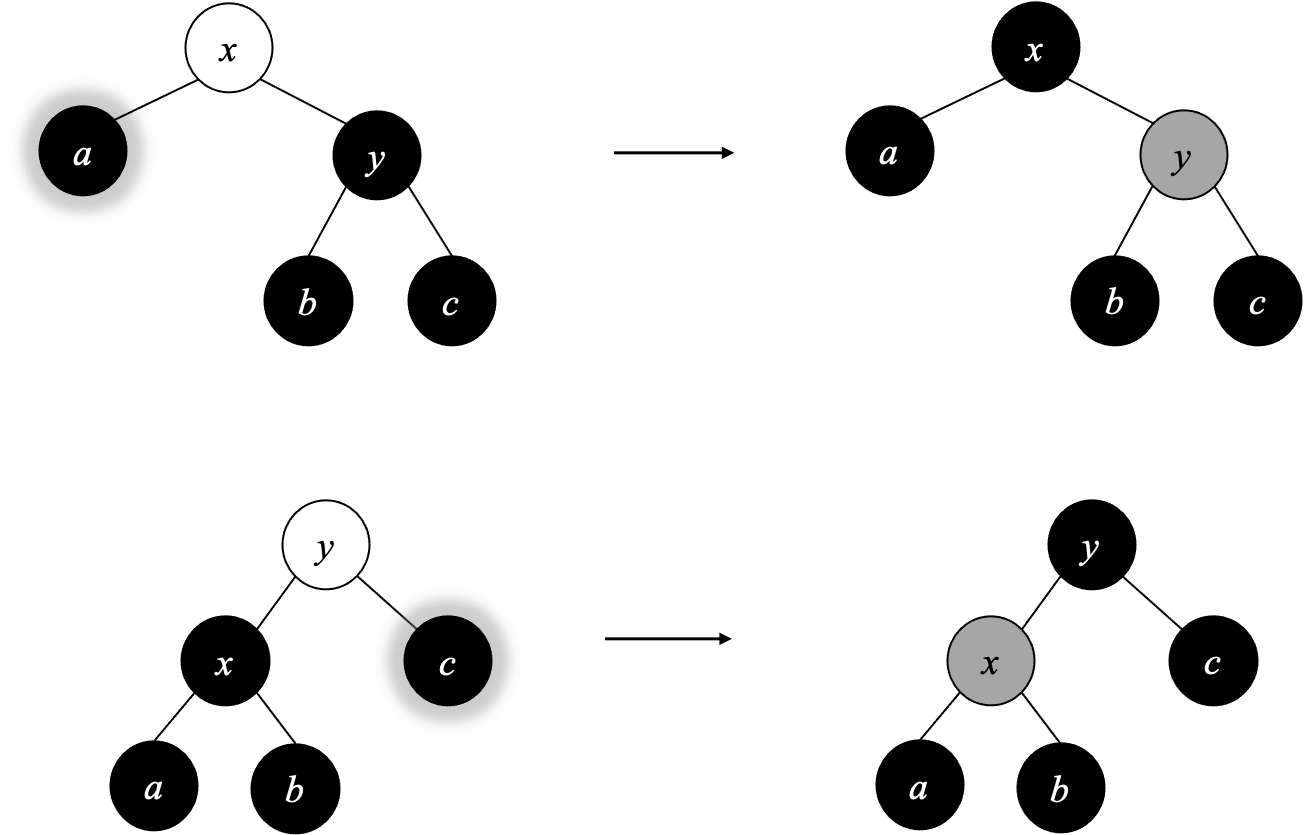
\includegraphics[scale=0.4]{img/del-case3.eps}
  \caption{The sibling of the doubly-black node is red.} \label{fig:del-case2}
\end{figure}

We can add this case on top of (\ref{eq:db-case-1a}) to gain (\ref{eq:db-case-2}).

\be
fixBlack^2(T) = \left \{
  \begin{array}
  {r@{\quad:\quad}l}
  ... & ... \\
  fixBlack^2(\mathcal{B}, fixBlack^2((\mathcal{R}, A, x, B), y, C) & p 2.1 \\
  fixBlack^2(\mathcal{B}, A, x, fixBlack^2((\mathcal{R}, B, y, C)) & p 2.2 \\
  T & otherwise
  \end{array}
\right .
\label{eq:db-case-2}
\ee

where $p 2.1$ and $p 2.2$ are two patterns as the following.

\[
p 2.1 : \{ color(T) = \mathcal{B} \land color(T_l) = \mathcal{B}^2 \land color(T_r) = \mathcal{R} \}
\]

\[
p 2.2 : \{ color(T) = \mathcal{B} \land color(T_l) = \mathcal{R} \land color(T_r) = \mathcal{B}^2 \}
\]

\subsection{The sibling of the doubly-black node, and its two children are all black}
In this case, we can change the color of the sibling node to red; turn the
doubly-black node to black and propagate the doubly-blackness one level
up to the parent node as shown in figure \ref{fig:del-case3}. There are two
symmetric sub-cases.

\begin{figure}[htbp]
  \centering
  \setlength{\unitlength}{1cm}
  \begin{picture}(10, 4)
  \put(5, 2){$\Longrightarrow$}
  \subcaptionbox{Color of $x$ can be either black or red.}{\includegraphics[scale=0.4]{img/case2-a.ps}}
  \subcaptionbox{If $x$ was red, then it becomes black, otherwise, it becomes doubly-black.}{\includegraphics[scale=0.4]{img/case2-a1.ps}}
  \end{picture}
  \\
  \begin{picture}(10, 5)
  \put(5, 2){$\Longrightarrow$}
  \subcaptionbox{Color of $y$ can be either black or red.}{\includegraphics[scale=0.4]{img/case2-b.ps}}
  \subcaptionbox{If $y$ was red, then it becomes black, otherwise, it becomes doubly-black.}{\includegraphics[scale=0.4]{img/case2-b1.ps}}
  \end{picture}
  \\
  \begin{picture}(1, 0.5)\end{picture} %pad
  \caption{propagate the blackness up.} \label{fig:del-case3}
\end{figure}

We go on adding this fixing after formula (\ref{eq:db-case-2}).

\be
fixBlack^2(T) = \left \{
  \begin{array}
  {r@{\quad:\quad}l}
  ... & ... \\
  mkBlk((\mathcal{C}, mkBlk(A), x, (\mathcal{R}, B, y, C))) & p 3.1 \\
  mkBlk((\mathcal{C}, (\mathcal{R}, A, x, B), y, mkBlk(C))) & p 3.2 \\
  ... & ...
  \end{array}
\right .
\label{eq:db-case-3}
\ee

where $p 3.1$ and $p 3.2$ are two patterns as below.

\[
p 3.1 : \left \{ \begin{array}{l}
  T = (\mathcal{C}, A, x, (\mathcal{B}, B, y, C)) \land \\
  color(A) = \mathcal{B}^2 \land color(B) = color(C) = \mathcal{B}
  \end{array} \right \}
\]

\[
p 3.2 : \left \{ \begin{array}{l}
  T = (\mathcal{C}, (\mathcal{B}, A, x, B), y, C) \land \\
  color(C) = \mathcal{B}^2 \land color(A) = color(B) = \mathcal{B}
  \end{array} \right \}
\]

If the doubly black node is doubly black empty node $\Phi$, it can be changed
back to normal empty node after re-coloring. We add the doubly black empty node
handling to (\ref{eq:db-case-3}) as below.

\be
fixBlack^2(T) = \left \{
  \begin{array}
  {r@{\quad:\quad}l}
  ... & ... \\
  mkBlk((\mathcal{C}, mkBlk(A), x, (\mathcal{R}, B, y, C))) & p 2.1 \\
  mkBlk((\mathcal{C}, \phi, x, (\mathcal{R}, B, y, C))) & p 2.1' \\
  mkBlk((\mathcal{C}, (\mathcal{R}, A, x, B), y, mkBlk(C))) & p 2.2 \\
  mkBlk((\mathcal{C}, (\mathcal{R}, A, x, B), y, \phi)) & p 2.2' \\
  ... & ...
  \end{array}
\right .
\label{eq:db-case-3a}
\ee

Where pattern $p 3.1'$ and $p 3.2'$ are defined as the following.

\[
p 3.1' : \left \{ \begin{array}{l}
  T = (\mathcal{C}, \Phi, x, (\mathcal{B}, B, y, C)) \land \\
  color(B) = color(C) = \mathcal{B}
  \end{array} \right \}
\]

\[
p 3.2' : \left \{ \begin{array}{l}
  T = (\mathcal{C}, (\mathcal{B}, A, x, B), y, \Phi) \land \\
  color(A) = color(B) = \mathcal{B}
  \end{array} \right \}
\]

Fixing the doubly-black node with all above different cases is a recursive function.
There are two termination conditions. One contains pattern $p 1.1$ and $p 1.2$,
The doubly-black node was eliminated. The other cases may continuously propagate the
doubly-blackness from bottom to top till the root.
Finally the algorithm marks the root node as black anyway. The doubly-blackness will be
removed.

Put formula (\ref{eq:db-case-1a}), (\ref{eq:db-case-2}), and (\ref{eq:db-case-3a})
together, we can write the final Haskell program.

\begin{lstlisting}
-- the sibling is black, and it has one red child
fixDB color a@(Node BB _ _ _) x (Node B (Node R b y c) z d)
      = Node color (Node B (makeBlack a) x b) y (Node B c z d)
fixDB color BBEmpty x (Node B (Node R b y c) z d)
      = Node color (Node B Empty x b) y (Node B c z d)
fixDB color a@(Node BB _ _ _) x (Node B b y (Node R c z d))
      = Node color (Node B (makeBlack a) x b) y (Node B c z d)
fixDB color BBEmpty x (Node B b y (Node R c z d))
      = Node color (Node B Empty x b) y (Node B c z d)
fixDB color (Node B a x (Node R b y c)) z d@(Node BB _ _ _)
      = Node color (Node B a x b) y (Node B c z (makeBlack d))
fixDB color (Node B a x (Node R b y c)) z BBEmpty
      = Node color (Node B a x b) y (Node B c z Empty)
fixDB color (Node B (Node R a x b) y c) z d@(Node BB _ _ _)
      = Node color (Node B a x b) y (Node B c z (makeBlack d))
fixDB color (Node B (Node R a x b) y c) z BBEmpty
      = Node color (Node B a x b) y (Node B c z Empty)
-- the sibling is red
fixDB B a@(Node BB _ _ _) x (Node R b y c) = fixDB B (fixDB R a x b) y c
fixDB B a@BBEmpty x (Node R b y c) = fixDB B (fixDB R a x b) y c
fixDB B (Node R a x b) y c@(Node BB _ _ _) = fixDB B a x (fixDB R b y c)
fixDB B (Node R a x b) y c@BBEmpty = fixDB B a x (fixDB R b y c)
-- the sibling and its 2 children are all black, propagate the blackness up
fixDB color a@(Node BB _ _ _) x (Node B b y c) = makeBlack (Node color (makeBlack a) x (Node R b y c))
fixDB color BBEmpty x (Node B b y c) = makeBlack (Node color Empty x (Node R b y c))
fixDB color (Node B a x b) y c@(Node BB _ _ _) = makeBlack (Node color (Node R a x b) y (makeBlack c))
fixDB color (Node B a x b) y BBEmpty = makeBlack (Node color (Node R a x b) y Empty)
-- otherwise
fixDB color l k r = Node color l k r
\end{lstlisting}

The deletion algorithm takes $O(\lg n)$ time to delete a key from
a red-black tree with $n$ nodes.

\begin{Exercise}

\begin{itemize}
\item As we mentioned in this section, deletion can be implemented
by just marking the node as deleted without actually removing it.
Once the number of marked nodes exceeds 50\%, a tree re-build is performed. Try to implement this
method in your favorite programming language.
\item Why needn't enclose $mkBlk$ with a call to $fixBlack^2$ explicitly in the definition of $del(T, k)$?
\end{itemize}

\end{Exercise}

\section{Imperative red-black tree algorithm $\star$}
\index{red-black tree!imperative insertion}

We almost finished all the content in this chapter. By induction
the patterns, we can implement the red-black tree in a simple way
compare to the imperative tree rotation solution. However, we
should show the comparator for completeness.

For insertion, the basic idea is to use the similar algorithm
as described in binary search tree. And then fix the balance
problem by rotation and return the final result.

\begin{algorithmic}[1]
\Function{Insert}{$T, k$}
  \State $root \gets T$
  \State $x \gets$ \Call{Create-Leaf}{$k$}
  \State \Call{Color}{$x$} $\gets$ RED
  \State $p \gets$ NIL
  \While{$T \neq$ NIL}
    \State $p \gets T$
    \If{$k <$ \Call{Key}{$T$}}
      \State $T \gets $ \Call{Left}{$T$}
    \Else
      \State $T \gets $ \Call{Right}{$T$}
    \EndIf
  \EndWhile
  \State \Call{Parent}{$x$} $\gets p$
  \If{$p =$ NIL} \Comment{tree $T$ is empty}
    \State \Return $x$
  \ElsIf{$k <$ \Call{Key}{$p$}}
    \State \Call{Left}{$p$} $\gets x$
  \Else
    \State \Call{Right}{$p$} $\gets x$
  \EndIf
  \State \Return \Call{Insert-Fix}{$root, x$}
\EndFunction
\end{algorithmic}

The only difference from the binary search tree insertion algorithm
is that we set the color of the new node as red, and perform fixing
before return. Below is the example Python program.

\lstset{language=Python}
\begin{lstlisting}
def rb_insert(t, key):
    root = t
    x = Node(key)
    parent = None
    while(t):
        parent = t
        if(key < t.key):
            t = t.left
        else:
            t = t.right
    if parent is None: #tree is empty
        root = x
    elif key < parent.key:
        parent.set_left(x)
    else:
        parent.set_right(x)
    return rb_insert_fix(root, x)
\end{lstlisting}

There are 3 base cases for fixing, and if we take the left-right
symmetric into consideration. there are total 6 cases.
Among them two cases can be merged together, because they all have
uncle node in red color, we can toggle the parent color and
uncle color to black and set grand parent color to red.
With this merging, the fixing algorithm can be realized as the following.

\begin{algorithmic}[1]
\Function{Insert-Fix}{$T, x$}
  \While{\Call{Parent}{$x$} $\neq$ NIL $\land$ \textproc{Color}(\Call{Parent}{$x$}) = RED}
    \If{\textproc{Color}(\Call{Uncle}{$x$}) $=$ RED}
      \Comment{Case 1, x's uncle is red}
      \State \textproc{Color}(\Call{Parent}{$x$}) $\gets$ BLACK
      \State \textproc{Color}(\Call{Grand-Parent}{$x$}) $\gets$ RED
      \State \textproc{Color}(\Call{Uncle}{$x$}) $\gets$ BLACK
      \State $x \gets$ \Call{Grand-Parent}{$x$}
    \Else
      \Comment{x's uncle is black}
      \If{\Call{Parent}{$x$} = \textproc{Left}(\Call{Grand-Parent}{$x$})}
        \If{ $x =$ \textproc{Right}(\Call{Parent}{$x$})}
          \Comment{Case 2, x is a right child}
          \State $x \gets$ \Call{Parent}{$x$}
          \State $T \gets$ \Call{Left-Rotate}{$T, x$}
        \EndIf
        \Comment{Case 3, x is a left child}
        \State \textproc{Color}(\Call{Parent}{$x$}) $\gets$ BLACK
        \State \textproc{Color}(\Call{Grand-Parent}{$x$}) $\gets$ RED
        \State $T \gets$ \textproc{Right-Rotate}($T$, \Call{Grand-Parent}{$x$})
      \Else
         \If{ $x =$ \textproc{Left}(\Call{Parent}{$x$})}
          \Comment{Case 2, Symmetric}
          \State $x \gets$ \Call{Parent}{$x$}
          \State $T \gets$ \Call{Right-Rotate}{$T, x$}
        \EndIf
        \Comment{Case 3, Symmetric}
        \State \textproc{Color}(\Call{Parent}{$x$}) $\gets$ BLACK
        \State \textproc{Color}(\Call{Grand-Parent}{$x$}) $\gets$ RED
        \State $T \gets$ \textproc{Left-Rotate}($T$, \Call{Grand-Parent}{$x$})
      \EndIf
    \EndIf
  \EndWhile
  \State \Call{Color}{$T$} $\gets$ BLACK
  \State \Return $T$
\EndFunction
\end{algorithmic}

This program takes $O(\lg n)$ time to insert a new key to the red-black tree.
Compare this pseudo code and the $balance$ function we defined in previous
section, we can see the difference. They differ not only in terms of
simplicity, but also in logic. Even if we feed the same series of keys to
the two algorithms, they may build different red-black trees. There
is a bit performance overhead in the pattern matching algorithm.
Okasaki discussed about the difference in detail in his paper\cite{okasaki}.

Translate the above algorithm to Python yields the below program.

\begin{lstlisting}
# Fix the red->red violation
def rb_insert_fix(t, x):
    while(x.parent and x.parent.color==RED):
        if x.uncle().color == RED:
            #case 1: ((a:R x:R b) y:B c:R) ==> ((a:R x:B b) y:R c:B)
            set_color([x.parent, x.grandparent(), x.uncle()],
                      [BLACK, RED, BLACK])
            x = x.grandparent()
        else:
            if x.parent == x.grandparent().left:
                if x == x.parent.right:
                    #case 2: ((a x:R b:R) y:B c) ==> case 3
                    x = x.parent
                    t=left_rotate(t, x)
                # case 3: ((a:R x:R b) y:B c) ==> (a:R x:B (b y:R c))
                set_color([x.parent, x.grandparent()], [BLACK, RED])
                t=right_rotate(t, x.grandparent())
            else:
                if x == x.parent.left:
                    #case 2': (a x:B (b:R y:R c)) ==> case 3'
                    x = x.parent
                    t = right_rotate(t, x)
                # case 3': (a x:B (b y:R c:R)) ==> ((a x:R b) y:B c:R)
                set_color([x.parent, x.grandparent()], [BLACK, RED])
                t=left_rotate(t, x.grandparent())
    t.color = BLACK
    return t
\end{lstlisting}

Figure \ref{fig:imperative-insert} shows the results of feeding same
series of keys to the above python insertion program. Compare them with
figure \ref{fig:insert-example}, one can tell the difference clearly.

\begin{figure}[htbp]
   \centering
   \subcaptionbox{}{\includegraphics[scale=0.4]{img/clrs-fig-13-4.ps}}
   \subcaptionbox{}{\includegraphics[scale=0.4]{img/python-insert.ps}}
   \caption{Red-black trees created by imperative algorithm.}
   \label{fig:imperative-insert}
\end{figure}

We put the red-black tree delete algorithm in imperative settings in Appendix B,
because it is more complex than the insertion.

\section{More words}
Red-black tree is the most popular implementation of balanced binary search
tree. Another one is the AVL tree, which we'll introduce in next chapter.
Red-black tree can be a good start point for more data structures. If we
extend the number of children from 2 to $k$, and keep the balance as well,
it leads to B-tree, If we store the data along with edge but not inside
node, it leads to Tries. However, the multiple cases handling and the long
program tends to make new comers think red-black tree is complex.

Okasaki's work helps making the red-black tree much easily understand.
There are many implementation in other programming languages in that
manner \cite{rosetta}. It's also inspired me to find the pattern matching
solution for Splay tree and AVL tree etc.

\section{Appendix: Example programs}

Definition of red-black tree node with parent field. When not explicitly defined, the color of the new node is red by default.

\begin{lstlisting}[language = Bourbaki]
data Node<T> {
    T key
    Color color
    Node<T> left
    Node<T> right
    Node<T> parent

    Node(T x) = Node(null, x, null, Color.RED)

    Node(Node<T> l, T k, Node<T> r, Color c) {
        left = l, key = k, right = r, color = c
        if (left != null) then left.parent = this
        if (right != null) then right.parent = this
    }
}
\end{lstlisting}

\begin{thebibliography}{99}

\bibitem{CLRS}
Thomas H. Cormen, Charles E. Leiserson, Ronald L. Rivest and Clifford Stein.
``Introduction to Algorithms, Second Edition''. ISBN:0262032937. The MIT Press. 2001

\bibitem{okasaki}
Chris Okasaki. ``FUNCTIONAL PEARLS Red-Black Trees in a Functional Setting''. J. Functional Programming. 1998

\bibitem{okasaki-blog}
Chris Okasaki. ``Ten Years of Purely Functional Data Structures''. http://okasaki.blogspot.com/2008/02/ten-years-of-purely-functional-data.html

\bibitem{wiki-rbt}
Wikipedia. ``Red-black tree''. \url{http://en.wikipedia.org/wiki/Red-black\_tree}

\bibitem{rosetta}
Pattern matching. \url{http://rosettacode.org/wiki/Pattern\_matching}

\end{thebibliography}

\ifx\wholebook\relax\else
\end{document}
\fi
